% Options for packages loaded elsewhere
\PassOptionsToPackage{unicode}{hyperref}
\PassOptionsToPackage{hyphens}{url}
\PassOptionsToPackage{dvipsnames,svgnames,x11names}{xcolor}
%
\documentclass[
]{agujournal2019}

\usepackage{amsmath,amssymb}
\usepackage{iftex}
\ifPDFTeX
  \usepackage[T1]{fontenc}
  \usepackage[utf8]{inputenc}
  \usepackage{textcomp} % provide euro and other symbols
\else % if luatex or xetex
  \usepackage{unicode-math}
  \defaultfontfeatures{Scale=MatchLowercase}
  \defaultfontfeatures[\rmfamily]{Ligatures=TeX,Scale=1}
\fi
\usepackage{lmodern}
\ifPDFTeX\else  
    % xetex/luatex font selection
\fi
% Use upquote if available, for straight quotes in verbatim environments
\IfFileExists{upquote.sty}{\usepackage{upquote}}{}
\IfFileExists{microtype.sty}{% use microtype if available
  \usepackage[]{microtype}
  \UseMicrotypeSet[protrusion]{basicmath} % disable protrusion for tt fonts
}{}
\makeatletter
\@ifundefined{KOMAClassName}{% if non-KOMA class
  \IfFileExists{parskip.sty}{%
    \usepackage{parskip}
  }{% else
    \setlength{\parindent}{0pt}
    \setlength{\parskip}{6pt plus 2pt minus 1pt}}
}{% if KOMA class
  \KOMAoptions{parskip=half}}
\makeatother
\usepackage{xcolor}
\setlength{\emergencystretch}{3em} % prevent overfull lines
\setcounter{secnumdepth}{5}
% Make \paragraph and \subparagraph free-standing
\makeatletter
\ifx\paragraph\undefined\else
  \let\oldparagraph\paragraph
  \renewcommand{\paragraph}{
    \@ifstar
      \xxxParagraphStar
      \xxxParagraphNoStar
  }
  \newcommand{\xxxParagraphStar}[1]{\oldparagraph*{#1}\mbox{}}
  \newcommand{\xxxParagraphNoStar}[1]{\oldparagraph{#1}\mbox{}}
\fi
\ifx\subparagraph\undefined\else
  \let\oldsubparagraph\subparagraph
  \renewcommand{\subparagraph}{
    \@ifstar
      \xxxSubParagraphStar
      \xxxSubParagraphNoStar
  }
  \newcommand{\xxxSubParagraphStar}[1]{\oldsubparagraph*{#1}\mbox{}}
  \newcommand{\xxxSubParagraphNoStar}[1]{\oldsubparagraph{#1}\mbox{}}
\fi
\makeatother

\usepackage{color}
\usepackage{fancyvrb}
\newcommand{\VerbBar}{|}
\newcommand{\VERB}{\Verb[commandchars=\\\{\}]}
\DefineVerbatimEnvironment{Highlighting}{Verbatim}{commandchars=\\\{\}}
% Add ',fontsize=\small' for more characters per line
\usepackage{framed}
\definecolor{shadecolor}{RGB}{241,243,245}
\newenvironment{Shaded}{\begin{snugshade}}{\end{snugshade}}
\newcommand{\AlertTok}[1]{\textcolor[rgb]{0.68,0.00,0.00}{#1}}
\newcommand{\AnnotationTok}[1]{\textcolor[rgb]{0.37,0.37,0.37}{#1}}
\newcommand{\AttributeTok}[1]{\textcolor[rgb]{0.40,0.45,0.13}{#1}}
\newcommand{\BaseNTok}[1]{\textcolor[rgb]{0.68,0.00,0.00}{#1}}
\newcommand{\BuiltInTok}[1]{\textcolor[rgb]{0.00,0.23,0.31}{#1}}
\newcommand{\CharTok}[1]{\textcolor[rgb]{0.13,0.47,0.30}{#1}}
\newcommand{\CommentTok}[1]{\textcolor[rgb]{0.37,0.37,0.37}{#1}}
\newcommand{\CommentVarTok}[1]{\textcolor[rgb]{0.37,0.37,0.37}{\textit{#1}}}
\newcommand{\ConstantTok}[1]{\textcolor[rgb]{0.56,0.35,0.01}{#1}}
\newcommand{\ControlFlowTok}[1]{\textcolor[rgb]{0.00,0.23,0.31}{\textbf{#1}}}
\newcommand{\DataTypeTok}[1]{\textcolor[rgb]{0.68,0.00,0.00}{#1}}
\newcommand{\DecValTok}[1]{\textcolor[rgb]{0.68,0.00,0.00}{#1}}
\newcommand{\DocumentationTok}[1]{\textcolor[rgb]{0.37,0.37,0.37}{\textit{#1}}}
\newcommand{\ErrorTok}[1]{\textcolor[rgb]{0.68,0.00,0.00}{#1}}
\newcommand{\ExtensionTok}[1]{\textcolor[rgb]{0.00,0.23,0.31}{#1}}
\newcommand{\FloatTok}[1]{\textcolor[rgb]{0.68,0.00,0.00}{#1}}
\newcommand{\FunctionTok}[1]{\textcolor[rgb]{0.28,0.35,0.67}{#1}}
\newcommand{\ImportTok}[1]{\textcolor[rgb]{0.00,0.46,0.62}{#1}}
\newcommand{\InformationTok}[1]{\textcolor[rgb]{0.37,0.37,0.37}{#1}}
\newcommand{\KeywordTok}[1]{\textcolor[rgb]{0.00,0.23,0.31}{\textbf{#1}}}
\newcommand{\NormalTok}[1]{\textcolor[rgb]{0.00,0.23,0.31}{#1}}
\newcommand{\OperatorTok}[1]{\textcolor[rgb]{0.37,0.37,0.37}{#1}}
\newcommand{\OtherTok}[1]{\textcolor[rgb]{0.00,0.23,0.31}{#1}}
\newcommand{\PreprocessorTok}[1]{\textcolor[rgb]{0.68,0.00,0.00}{#1}}
\newcommand{\RegionMarkerTok}[1]{\textcolor[rgb]{0.00,0.23,0.31}{#1}}
\newcommand{\SpecialCharTok}[1]{\textcolor[rgb]{0.37,0.37,0.37}{#1}}
\newcommand{\SpecialStringTok}[1]{\textcolor[rgb]{0.13,0.47,0.30}{#1}}
\newcommand{\StringTok}[1]{\textcolor[rgb]{0.13,0.47,0.30}{#1}}
\newcommand{\VariableTok}[1]{\textcolor[rgb]{0.07,0.07,0.07}{#1}}
\newcommand{\VerbatimStringTok}[1]{\textcolor[rgb]{0.13,0.47,0.30}{#1}}
\newcommand{\WarningTok}[1]{\textcolor[rgb]{0.37,0.37,0.37}{\textit{#1}}}

\providecommand{\tightlist}{%
  \setlength{\itemsep}{0pt}\setlength{\parskip}{0pt}}\usepackage{longtable,booktabs,array}
\usepackage{calc} % for calculating minipage widths
% Correct order of tables after \paragraph or \subparagraph
\usepackage{etoolbox}
\makeatletter
\patchcmd\longtable{\par}{\if@noskipsec\mbox{}\fi\par}{}{}
\makeatother
% Allow footnotes in longtable head/foot
\IfFileExists{footnotehyper.sty}{\usepackage{footnotehyper}}{\usepackage{footnote}}
\makesavenoteenv{longtable}
\usepackage{graphicx}
\makeatletter
\newsavebox\pandoc@box
\newcommand*\pandocbounded[1]{% scales image to fit in text height/width
  \sbox\pandoc@box{#1}%
  \Gscale@div\@tempa{\textheight}{\dimexpr\ht\pandoc@box+\dp\pandoc@box\relax}%
  \Gscale@div\@tempb{\linewidth}{\wd\pandoc@box}%
  \ifdim\@tempb\p@<\@tempa\p@\let\@tempa\@tempb\fi% select the smaller of both
  \ifdim\@tempa\p@<\p@\scalebox{\@tempa}{\usebox\pandoc@box}%
  \else\usebox{\pandoc@box}%
  \fi%
}
% Set default figure placement to htbp
\def\fps@figure{htbp}
\makeatother
% definitions for citeproc citations
\NewDocumentCommand\citeproctext{}{}
\NewDocumentCommand\citeproc{mm}{%
  \begingroup\def\citeproctext{#2}\cite{#1}\endgroup}
\makeatletter
 % allow citations to break across lines
 \let\@cite@ofmt\@firstofone
 % avoid brackets around text for \cite:
 \def\@biblabel#1{}
 \def\@cite#1#2{{#1\if@tempswa , #2\fi}}
\makeatother
\newlength{\cslhangindent}
\setlength{\cslhangindent}{1.5em}
\newlength{\csllabelwidth}
\setlength{\csllabelwidth}{3em}
\newenvironment{CSLReferences}[2] % #1 hanging-indent, #2 entry-spacing
 {\begin{list}{}{%
  \setlength{\itemindent}{0pt}
  \setlength{\leftmargin}{0pt}
  \setlength{\parsep}{0pt}
  % turn on hanging indent if param 1 is 1
  \ifodd #1
   \setlength{\leftmargin}{\cslhangindent}
   \setlength{\itemindent}{-1\cslhangindent}
  \fi
  % set entry spacing
  \setlength{\itemsep}{#2\baselineskip}}}
 {\end{list}}
\usepackage{calc}
\newcommand{\CSLBlock}[1]{\hfill\break\parbox[t]{\linewidth}{\strut\ignorespaces#1\strut}}
\newcommand{\CSLLeftMargin}[1]{\parbox[t]{\csllabelwidth}{\strut#1\strut}}
\newcommand{\CSLRightInline}[1]{\parbox[t]{\linewidth - \csllabelwidth}{\strut#1\strut}}
\newcommand{\CSLIndent}[1]{\hspace{\cslhangindent}#1}

\usepackage{url} %this package should fix any errors with URLs in refs.
\usepackage{lineno}
\usepackage[inline]{trackchanges} %for better track changes. finalnew option will compile document with changes incorporated.
\usepackage{soul}
\linenumbers
\makeatletter
\@ifpackageloaded{caption}{}{\usepackage{caption}}
\AtBeginDocument{%
\ifdefined\contentsname
  \renewcommand*\contentsname{Table of contents}
\else
  \newcommand\contentsname{Table of contents}
\fi
\ifdefined\listfigurename
  \renewcommand*\listfigurename{List of Figures}
\else
  \newcommand\listfigurename{List of Figures}
\fi
\ifdefined\listtablename
  \renewcommand*\listtablename{List of Tables}
\else
  \newcommand\listtablename{List of Tables}
\fi
\ifdefined\figurename
  \renewcommand*\figurename{Figure}
\else
  \newcommand\figurename{Figure}
\fi
\ifdefined\tablename
  \renewcommand*\tablename{Table}
\else
  \newcommand\tablename{Table}
\fi
}
\@ifpackageloaded{float}{}{\usepackage{float}}
\floatstyle{ruled}
\@ifundefined{c@chapter}{\newfloat{codelisting}{h}{lop}}{\newfloat{codelisting}{h}{lop}[chapter]}
\floatname{codelisting}{Listing}
\newcommand*\listoflistings{\listof{codelisting}{List of Listings}}
\makeatother
\makeatletter
\makeatother
\makeatletter
\@ifpackageloaded{caption}{}{\usepackage{caption}}
\@ifpackageloaded{subcaption}{}{\usepackage{subcaption}}
\makeatother

\usepackage{bookmark}

\IfFileExists{xurl.sty}{\usepackage{xurl}}{} % add URL line breaks if available
\urlstyle{same} % disable monospaced font for URLs
\hypersetup{
  pdftitle={Supply Chain Data Analytics},
  colorlinks=true,
  linkcolor={blue},
  filecolor={Maroon},
  citecolor={Blue},
  urlcolor={Blue},
  pdfcreator={LaTeX via pandoc}}


\journalname{Earth and Space Science}

\draftfalse

\begin{document}
\title{Supply Chain Data Analytics}

\authors{Stan Brouwer\affil{1}, Liz Chan\affil{2}, Maaike
Lamberst\affil{3}, Niek Schroor\affil{4}}
\affiliation{1}{Vrije Universiteit, }\affiliation{2}{Master
TSCM, }\affiliation{3}{Supply Chain Data
analysis, }\affiliation{4}{Group 10, }
\correspondingauthor{Stan Brouwer}{}







Introduction

We analyze, forecast and interpret the
\href{https://public.tableau.com/app/sample-data/sample_-_superstore.xls}{Superstore
sales} provided by
\href{https://public.tableau.com/app/learn/sample-data}{Tableau} using
different statistical and machine learning methods.

We describe our work in the PDF version. However, we would like to
recommend reading our quarto manuscript \emph{here} as it contains the
\textbf{relevant} R code in the Article Notebook.

\subsection{Data Pre-processing}\label{data-pre-processing}

The superstore data set we selected is of high quality. Thus we do the
required data pre-processing, but included the hypothetical steps we
would take were our data of lower quality to communicate our
understanding of the data pre-processing process.

We took the following pre-processing steps:

\begin{itemize}
\tightlist
\item
  Improved column names by removing whitespaces
\item
  Removed the Row\_ID column as it can be inferred by it's index
\item
  Removed all columns with a single unique value, as storing these would
  be
  \href{https://few.vu.nl/~molenaar/courses/StatR/chapters/B-06-raw_data.html}{redundant}
\item
  Ensured machine-readable date formats in yyyy-mm-dd as these usually
  differ per locale.
\item
  Ensured proper decimal separators
\item
  Calculated the number of missing values (both NA and empty string
  ``\,``) per column.
\end{itemize}

\begin{verbatim}
[1] "None of the columns contains missing values"
\end{verbatim}

\textsubscript{Source:
\href{https://SJbrou.github.io/Supply_Chain_Data_Analysis/index.qmd.html}{Article
Notebook}}

After these steps (and transposing the table for better document
formatting), the data looks as follows:

\begin{longtable}[]{@{}
  >{\raggedright\arraybackslash}p{(\linewidth - 6\tabcolsep) * \real{0.0843}}
  >{\raggedright\arraybackslash}p{(\linewidth - 6\tabcolsep) * \real{0.2048}}
  >{\raggedright\arraybackslash}p{(\linewidth - 6\tabcolsep) * \real{0.3614}}
  >{\raggedright\arraybackslash}p{(\linewidth - 6\tabcolsep) * \real{0.3494}}@{}}
\caption{First 5 Rows of the Data (Transposed)}\tabularnewline
\toprule\noalign{}
\endfirsthead
\endhead
\bottomrule\noalign{}
\endlastfoot
Order\_ID & CA-2016-152156 & CA-2016-152156 & CA-2016-138688 \\
Order\_Date & 2016-11-08 & 2016-11-08 & 2016-06-12 \\
Ship\_Date & 2016-11-11 & 2016-11-11 & 2016-06-16 \\
Ship\_Mode & Second Class & Second Class & Second Class \\
Customer\_ID & CG-12520 & CG-12520 & DV-13045 \\
Customer\_Name & Claire Gute & Claire Gute & Darrin Van Huff \\
Segment & Consumer & Consumer & Corporate \\
City & Henderson & Henderson & Los Angeles \\
State & Kentucky & Kentucky & California \\
Postal\_Code & 42420 & 42420 & 90036 \\
Region & South & South & West \\
Product\_ID & FUR-BO-10001798 & FUR-CH-10000454 & OFF-LA-10000240 \\
Category & Furniture & Furniture & Office Supplies \\
Sub-Category & Bookcases & Chairs & Labels \\
Product\_Name & Bush Somerset Collection Bookcase & Hon Deluxe Fabric
Upholstered Stacking Chairs, Rounded Back & Self-Adhesive Address Labels
for Typewriters by Universal \\
Sales & 261.96 & 731.94 & 14.62 \\
Quantity & 2 & 3 & 2 \\
Discount & 0 & 0 & 0 \\
Profit & 41.9136 & 219.5820 & 6.8714 \\
\end{longtable}

\textsubscript{Source:
\href{https://SJbrou.github.io/Supply_Chain_Data_Analysis/index.qmd.html}{Article
Notebook}}

There is some more processing to do, for instance the removing of
outliers. However, by doing so we impose our own assumptions on the
data. Let's start by evaluating the descriptive statistics of our data
and check if further processing is required.

\begin{longtable}[]{@{}llllll@{}}
\caption{Descriptive Statistics for Numeric Columns}\tabularnewline
\toprule\noalign{}
Column & Min & Max & Mean & Median & StdDev \\
\midrule\noalign{}
\endfirsthead
\toprule\noalign{}
Column & Min & Max & Mean & Median & StdDev \\
\midrule\noalign{}
\endhead
\bottomrule\noalign{}
\endlastfoot
Postal\_Code & 1040 & 99301 & 55190.38 & 56430.5 & 32063.69 \\
Sales & 0.444 & 22638.48 & 229.858 & 54.49 & 623.2451 \\
Quantity & 1 & 14 & 3.789574 & 3 & 2.22511 \\
Discount & 0 & 0.8 & 0.1562027 & 0.2 & 0.206452 \\
Profit & -6599.978 & 8399.976 & 28.6569 & 8.6665 & 234.2601 \\
\end{longtable}

\begin{longtable}[]{@{}lll@{}}
\caption{Descriptive Statistics for Date Columns}\tabularnewline
\toprule\noalign{}
Column & Earliest & Latest \\
\midrule\noalign{}
\endfirsthead
\toprule\noalign{}
Column & Earliest & Latest \\
\midrule\noalign{}
\endhead
\bottomrule\noalign{}
\endlastfoot
Order\_Date & 2014-01-03 & 2017-12-30 \\
Ship\_Date & 2014-01-07 & 2018-01-05 \\
\end{longtable}

\textsubscript{Source:
\href{https://SJbrou.github.io/Supply_Chain_Data_Analysis/index.qmd.html}{Article
Notebook}}

We inspected the orders with the lowest and highers price (Sales in
USD). The most expensive orders were professional printers, camera's and
teleconferencing units with high unit prices, and these orders often
were of high Quantity. The orders with the lowest price where often
binders, had a high Discount rate, and often a Quantity of just one.

We were fascinated by the orders with a negative profit. These all had
high Discount rates, and often concerned the same items, such as the
Cubify CubeX 3D Printer Triple Head Print. The orders with a negative
Profit where often part of a larger order (for instance CA-2016-108196),
and placed by customers that placed multiple orders. We suspect these
negative Profit's to be caused by faulty items that receive discounts,
general discount codes, or volumne discounts. However, due to especially
the high discounts on orders with negative profits, we assume these to
be valid orders. This decision has also been influenced by the high
quality of the data. As we found no missing values whatshowever, we
suspect the chance of some weird but valid orders to be higher than
encountering mistakes here. \emph{{[}this paragraph could use some
rewriting{]}}

\subsection{Data Visualization}\label{data-visualization}

\begin{verbatim}
# A tibble: 20 x 3
   Product_Name                                         total_quantity ProdName8
   <chr>                                                         <dbl> <chr>    
 1 Staples                                                         215 "Staples"
 2 Staple envelope                                                 170 "Staple ~
 3 Easy-staple paper                                               150 "Easy-st~
 4 Staples in misc. colors                                          86 "Staples~
 5 KI Adjustable-Height Table                                       74 "KI Adju~
 6 Avery Non-Stick Binders                                          71 "Avery N~
 7 Storex Dura Pro Binders                                          71 "Storex ~
 8 GBC Premium Transparent Covers with Diagonal Lined ~             67 "GBC Pre~
 9 Situations Contoured Folding Chairs, 4/Set                       64 "Situati~
10 Staple-based wall hangings                                       62 "Staple-~
11 Chromcraft Round Conference Tables                               61 "Chromcr~
12 Eldon Wave Desk Accessories                                      61 "Eldon W~
13 Staple remover                                                   61 "Staple ~
14 Global Wood Trimmed Manager's Task Chair, Khaki                  59 "Global ~
15 Wilson Jones Turn Tabs Binder Tool for Ring Binders              59 "Wilson ~
16 Kingston Digital DataTraveler 16GB USB 2.0                       57 "Kingsto~
17 Fellowes Officeware Wire Shelving                                55 "Fellowe~
18 Global High-Back Leather Tilter, Burgundy                        54 "Global ~
19 SAFCO Arco Folding Chair                                         53 "SAFCO A~
20 Xerox 226                                                        53 "Xerox 2~
\end{verbatim}

\pandocbounded{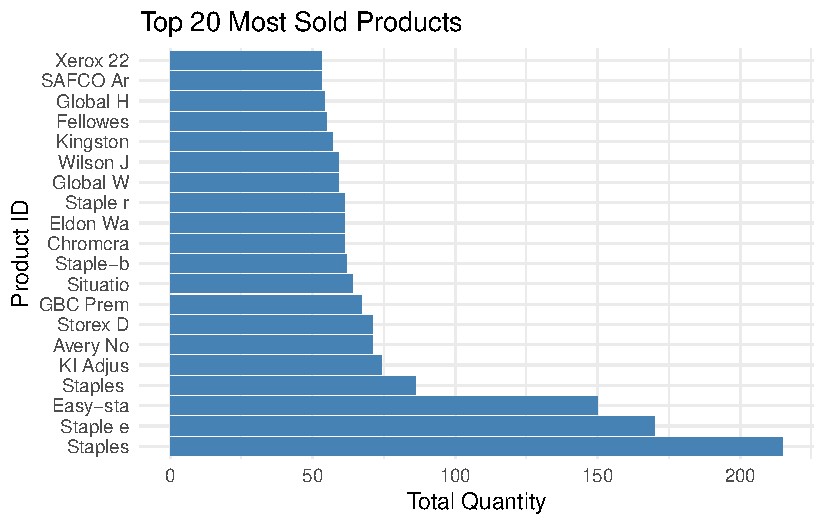
\includegraphics[keepaspectratio]{index_files/figure-pdf/data_viz1-1.pdf}}

\pandocbounded{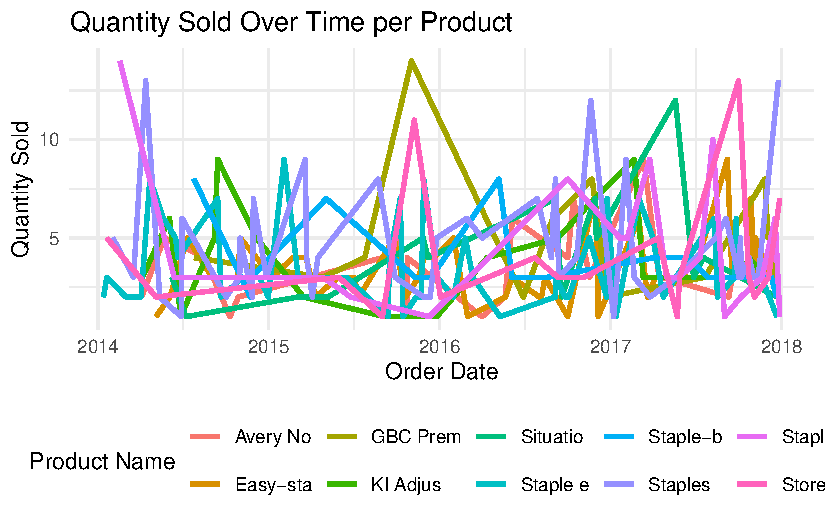
\includegraphics[keepaspectratio]{index_files/figure-pdf/data_viz1-2.pdf}}

\pandocbounded{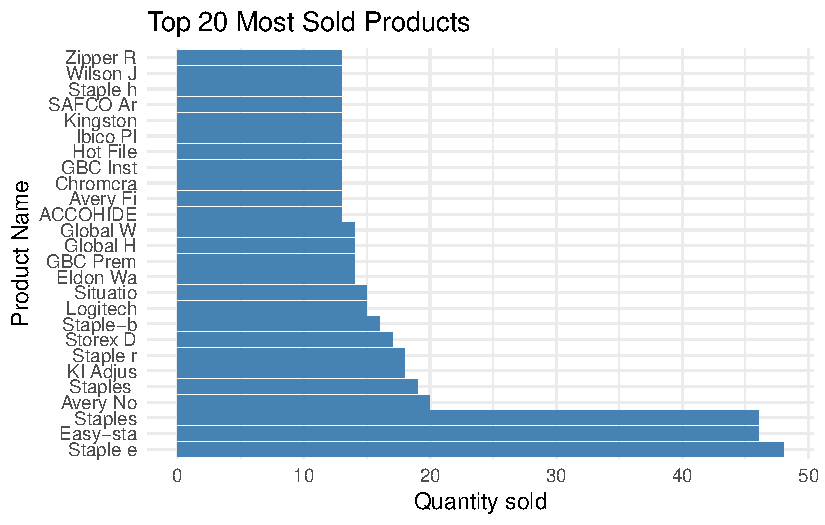
\includegraphics[keepaspectratio]{index_files/figure-pdf/data_viz1-3.pdf}}

\textsubscript{Source:
\href{https://SJbrou.github.io/Supply_Chain_Data_Analysis/index.qmd.html}{Article
Notebook}}

This is a simple placeholder for the manuscript's main document
(\textbf{knuth84?}).

\begin{Shaded}
\begin{Highlighting}[]
\DecValTok{1} \SpecialCharTok{+} \DecValTok{1}
\end{Highlighting}
\end{Shaded}

\begin{verbatim}
[1] 2
\end{verbatim}

\textsubscript{Source:
\href{https://SJbrou.github.io/Supply_Chain_Data_Analysis/index.qmd.html}{Article
Notebook}}

\subsection{Introduction}\label{introduction}

\textsubscript{Source:
\href{https://SJbrou.github.io/Supply_Chain_Data_Analysis/index.qmd.html}{Article
Notebook}}

\phantomsection\label{cell-fig-timeline}
\begin{figure}[H]

\centering{

\pandocbounded{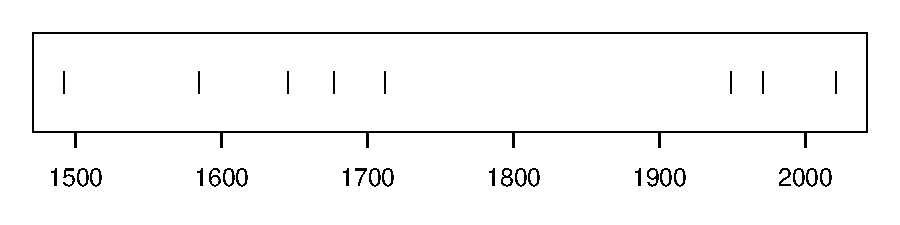
\includegraphics[keepaspectratio]{index_files/figure-pdf/fig-timeline-1.pdf}}

}

\caption{\label{fig-timeline}Timeline of recent earthquakes on La Palma}

\end{figure}%

\textsubscript{Source:
\href{https://SJbrou.github.io/Supply_Chain_Data_Analysis/index.qmd.html}{Article
Notebook}}

\textsubscript{Source:
\href{https://SJbrou.github.io/Supply_Chain_Data_Analysis/index.qmd.html}{Article
Notebook}}

Based on data up to and including 1971, eruptions on La Palma happen
every 79.8 years on average.

Studies of the magma systems feeding the volcano, such as Marrero et al.
(2019), have proposed that there are two main magma reservoirs feeding
the Cumbre Vieja volcano; one in the mantle (30-40km depth) which
charges and in turn feeds a shallower crustal reservoir (10-20km depth).

Eight eruptions have been recorded since the late 1400s
(Figure~\ref{fig-timeline}).

Data and methods are discussed in Section~\ref{sec-data-methods}.

Let \(x\) denote the number of eruptions in a year. Then, \(x\) can be
modeled by a Poisson distribution

\begin{equation}\phantomsection\label{eq-poisson}{
p(x) = \frac{e^{-\lambda} \lambda^{x}}{x !}
}\end{equation}

where \(\lambda\) is the rate of eruptions per year. Using
Equation~\ref{eq-poisson}, the probability of an eruption in the next
\(t\) years can be calculated.

\begin{longtable}[]{@{}ll@{}}
\caption{Recent historic eruptions on La
Palma}\label{tbl-history}\tabularnewline
\toprule\noalign{}
Name & Year \\
\midrule\noalign{}
\endfirsthead
\toprule\noalign{}
Name & Year \\
\midrule\noalign{}
\endhead
\bottomrule\noalign{}
\endlastfoot
Current & 2021 \\
Teneguía & 1971 \\
Nambroque & 1949 \\
El Charco & 1712 \\
Volcán San Antonio & 1677 \\
Volcán San Martin & 1646 \\
Tajuya near El Paso & 1585 \\
Montaña Quemada & 1492 \\
\end{longtable}

Table~\ref{tbl-history} summarises the eruptions recorded since the
colonization of the islands by Europeans in the late 1400s.

\begin{figure}

\centering{

\pandocbounded{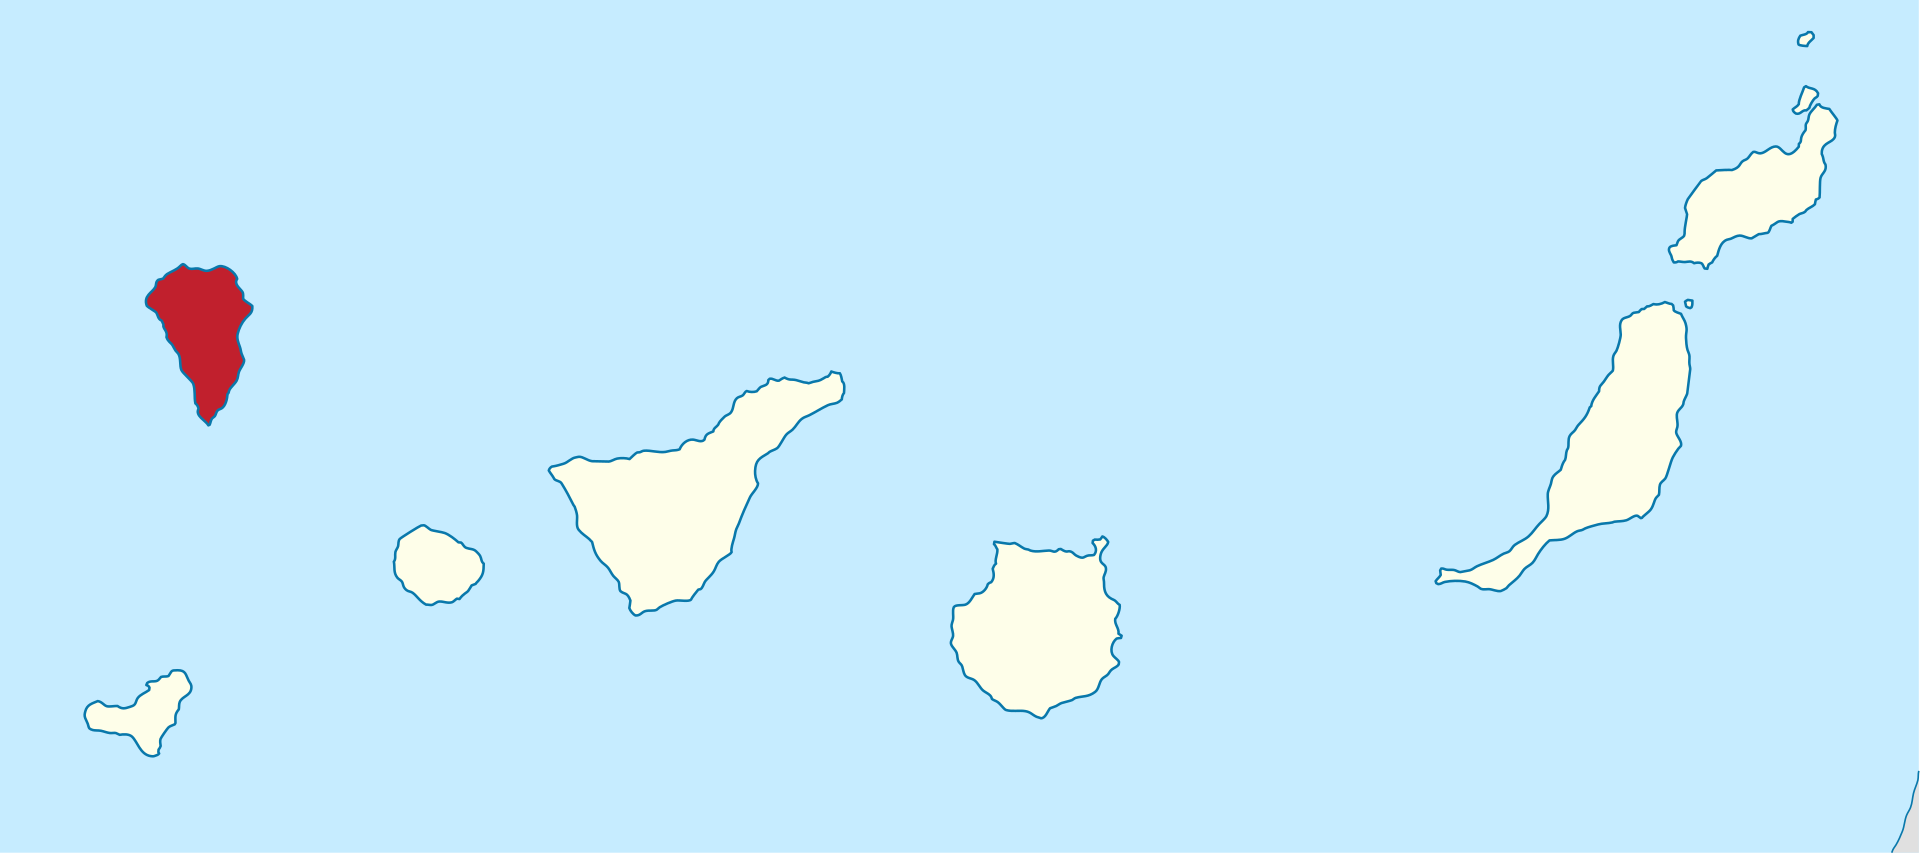
\includegraphics[keepaspectratio]{images/la-palma-map.png}}

}

\caption{\label{fig-map}Map of La Palma}

\end{figure}%

La Palma is one of the west most islands in the Volcanic Archipelago of
the Canary Islands (Figure~\ref{fig-map}).

\subsection{Data \& Methods}\label{sec-data-methods}

\subsection{Conclusion}\label{conclusion}

\subsection*{References}\label{references}
\addcontentsline{toc}{subsection}{References}

\phantomsection\label{refs}
\begin{CSLReferences}{1}{0}
\vspace{1em}

\bibitem[\citeproctext]{ref-marrero2019}
Marrero, J., García, A., Berrocoso, M., Llinares, Á., Rodríguez-Losada,
A., \& Ortiz, R. (2019). Strategies for the development of volcanic
hazard maps in monogenetic volcanic fields: The example of {La} {Palma}
({Canary} {Islands}). \emph{Journal of Applied Volcanology}, \emph{8}.
\url{https://doi.org/10.1186/s13617-019-0085-5}

\end{CSLReferences}




\end{document}
